\documentclass{article}
\usepackage{fullpage}
\usepackage[czech]{babel}
\usepackage{amsfonts}
\usepackage{amsmath}
\usepackage{graphicx}
\usepackage{caption}
\graphicspath{{images/}}

\title{\vspace{-2cm}Matouš Trnka swag\vspace{-1.7cm}}
\date{}
\author{}

\begin{document}
\maketitle

\part{Divná geometrie}

\section{Projektivní geometrie}

\subsection{Axiomy}
\begin{itemize}
  \item každé 2 body zadávají právě 1 přímku
  \item každé 2 přímky se protínají
  \item existují 3 body neležíí na jedné přímce
\end{itemize}
Z tohoto plyne:
\begin{itemize}
  \item každý bod má stejně přímek
  \item každá přímka má stejně bodů
  \item je stejně přímek jako bodů - $n^2+n+1$
\end{itemize}

\section{Afinní rovina}
\subsection{Axiomy}
\begin{itemize}
  \item stejné jako Projektivní geometrie, ale ne každé 2 přímky se musí potkat - existují ,,rovnoběžky" (právě jedna)
\end{itemize}
Takže:
\begin{itemize}
  \item každá přímka má stejný počet bodů - $n$
  \item každým bodem prochází stejně přímek - $n+1$
  \item celkem $n^2$ bodů, $n^2+n$ přímek
\end{itemize}
\subsection{Příklady}
VLOŽTE OBRÁZKY AFFINNÍCH ROVIN PRO N=1, 2, 3, 4
\begin{itemize}
  \item vždycky můžeme přímky afinní roviny rozdělit do $n$ kategorií rovnoběžnosti - že vždycky přímky z jedné kategorie jsou navzájem rovnoběžné (ekvivalentní relace)
\end{itemize}

\section{Latinské čtverce}
\subsection{Motivační úkol od Eulera}
\begin{itemize}
  \item Postavte do čtverce 36 důstojníků z 6 pluků o 6 hodnostech tak, aby v každém řádku i sloupci nebyl dvakrát stejný pluk ani hodnost.
\end{itemize}
VLOŽTE OBRÁZEK AAAA
\begin{itemize}
  \item nejde to lol
\end{itemize}
\subsection{Definice}
\begin{itemize}
  \item Je to $n*n$ čtverec, který musíme zaplnit prvky z $n$ kategorií tak, aby v žádném řádku ani sloupci nebyly dva prvky ze stejné kategorie.
\end{itemize}
\subsection{Počet možností}
\begin{itemize}
  \item Kolik je možností utvořit latinský čtverec pro dané $n$? Je jich $n!*(n-1)!*(n-2)!*...*1!$
  \item můžeme to spočítat pomocí perfektních párování bipartitních grafů
\end{itemize}
AAAAAA VYSVĚTLI TO MAGORE A OBRÁZEK NEJLÉPE
\subsection{Vraťme se}
\begin{itemize}
  \item Eulerův úkol můžeme vyřešit tak, že zkombinujeme 2 latinské čtverce
  \item což má nějakou souvislost s afinní rovinou
\end{itemize}
AAAAAAA vybil se mi počítač 1.3., tady zjevena souvislost s afinní rovinou

\part{Diferenční počet}

\section{Posloupnosti}
\begin{itemize}
  \item řada čísel idk, jakoby fce ale diskrétní, tj. počitatelné
\end{itemize}

\subsection{Definice}
\begin{itemize}
  \item předpisem - pro výpočet prvku je vzorec
  \item rekursí - pro výpočet prvku využíváme hodnoty předchozích prvků
  \item jako řešení diferenčních rcí (jakože diferenciální, ale diskrétní takže diferenční)
\end{itemize}

\subsection{Operátory na posloupnostech}
\begin{itemize}
  \item unární - potřebují jen jeden vstup, např. $\Delta$ (diference - rozdíl dvou prvků (derivace ekvivalent z fcí)), E (viz níže), umocnění/odmocnění, reciproká hodnota, atd.
  \item binární - potřebují dva vstupy, např. sčítání/odčítání, násobení/dělení, atd.
\end{itemize}

\subsection{Diference - $\Delta$}
$$\Delta a_n = a_{n+1} - a_n$$

\subsection{Shift operátor - E}
  $$E a_n = a_{n+1}$$
  Např. M = {1,2,3,...}, tak potom E M = {2,3,4,...}, můžeme dosadit do diference
  $$\Delta a_n = E a_n - a_n$$
  $$\Delta = E - 1$$ $\Rightarrow$ aritmetika operátorů (fokin pointery v programování, ale v matice) - nepočítám s číslama ale s operacema, tedy takto diference se rovná shift méně jedna, pomocí tohoto operátoru tedy můžeme vyjadřovat diference

\subsection{Příklady}
\begin{enumerate}
  \item rekurentní posloupnosti převést na předpis
  \item diferenční rovnice
\end{enumerate}
A zjišťujeme, že když převedem na shift operátor tak je to ten samý problém.

\section{Diferenční rovnice}
\begin{itemize}
  \item obecná nehomogenní řádu r: $$V(\Delta^r a_n, \Delta^{r-1} a_n,..., \Delta a_n, a_n, n) = 0$$ obecně neumíme řešit
  \item lineární homogenní diferenční rovnice s konstantními koeficienty: $$ k_r \Delta^r a_n + k_{r-1} \Delta^{r-1} a_n + ... + k_1 \Delta a_n + k_0 a_n = 0$$
\end{itemize}

\part{Vektorové prostory}
\section{Lineární zobrazení}
Def.: $\varphi: V \rightarrow U$ je lineární, jestliže:
\begin{itemize}
  \item $\varphi (x+y) = \varphi (x) + \varphi (y)$
  \item $\varphi (cx) = c \cdot \varphi (x)$
\end{itemize}

\part{nevim nějaký matice jako rotace}
\section{v $R^2$}
\begin{itemize}
  \item je to celkem zajímavý, dají se tak pěkně znázornit imag. čísla, pěkně definovat ostatní věci (norma, odchylka, vektorový součin) pomocí standardního skalarního součinu
\end{itemize}

\section{v $R^3$}
otázka: jak lze takovou rotaci charakterizovat? ano správně pomocí matice
1) Transformační matice
... báze $\alpha = (e_1, e_2, e_3)$
... rotace R
jak se píšou matice -- odporoučím se na papír

\part{4tvrtý ročník}

Def.: Relace $R$ je \textbf{uspořádání}, jestliže je:
\begin{enumerate}
  \item reflexivní: $aRa$
  \item antisymetrická: $aRb  \land bRa \implies a = b$
  \item tranzitivní: $aRb \land bRc \implies aRc$
\end{enumerate}

Každé uspořádání se dá zapsat pomocí tzv. \textbf{Hasseova diagramu}

\begin{figure}[h]
  \begin{center}
    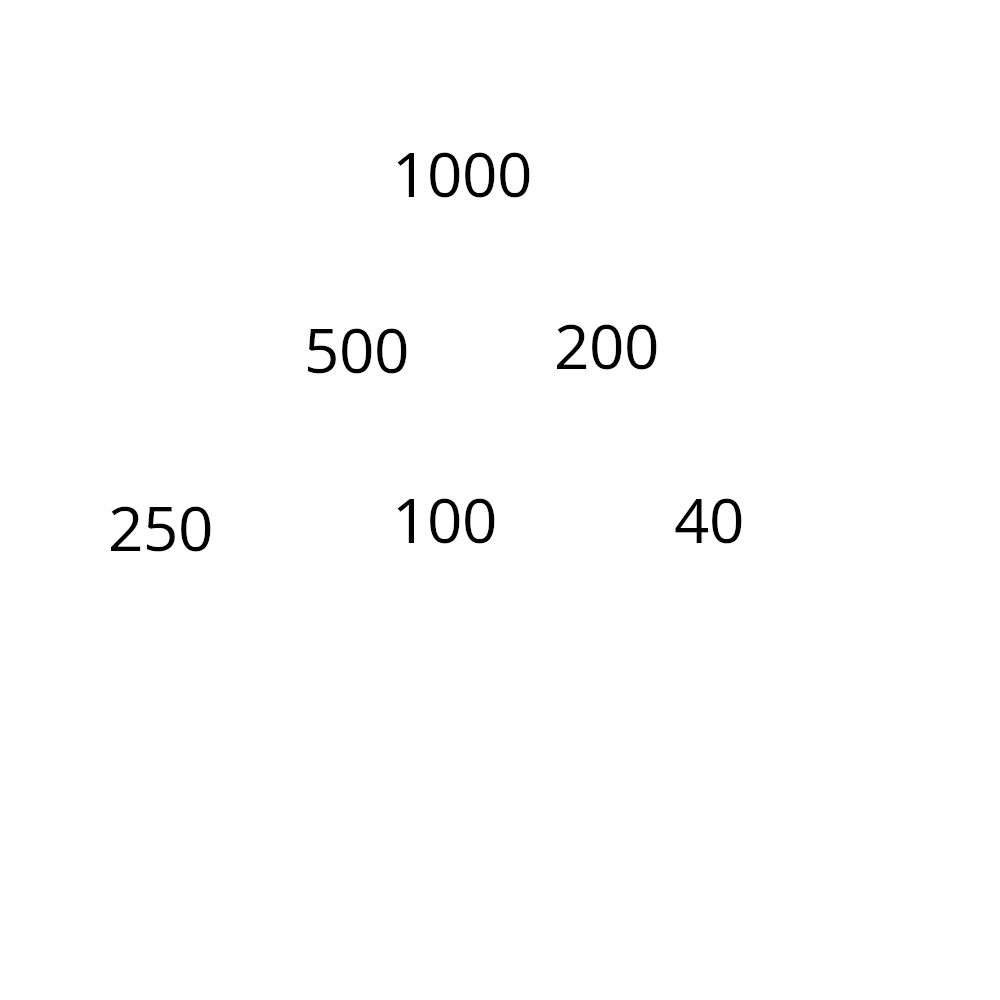
\includegraphics[width=0.5\textwidth]{hasseuv.png}
    \caption{Hasseův diagram relace \uv{dělí na $\mathbb N$} pro $1000$}
  \end{center}
\end{figure}



\end{document}
